\newpage
\chapter{Introduction}

\section{Background}
The exponential growth of digital media content over the past decade has created a critical need for robust and efficient content identification systems. Millions of audio and video files are shared, re-encoded, compressed, and re-distributed across platforms every day. Determining the original source of a short media snippet---even when it is noisy, cropped, or degraded---is a significant technical challenge with wide-ranging applications in digital rights management, forensic investigation, media archiving, and copyright enforcement.

Conventional file-comparison techniques such as cryptographic hashing (MD5, SHA-1) are entirely unsuitable for this purpose, as even a single-bit change in the file results in a completely different hash. What is required instead is a form of \textit{perceptual} or \textit{semantic} matching: identifying media by its content structure rather than its raw bytes.

Commercial solutions to this problem exist in the form of services such as Shazam (audio identification) and YouTube's Content ID (audio-visual identification). However, these systems are closed-source, cloud-dependent, and not accessible for educational or privacy-sensitive applications. There is a clear gap in the availability of locally deployable, transparent, and academically demonstrable media fingerprinting systems.

\section{Motivation}
This project is motivated by the desire to understand, replicate, and demonstrate the core algorithmic principles behind large-scale commercial content identification systems using publicly available tools and techniques.

\begin{enumerate}
  \item \textbf{Privacy and Sovereignty:} Cloud-based identification systems transmit user audio/video to remote servers. A local system eliminates this privacy concern.
  \item \textbf{Transparency:} Commercial systems are opaque. Mitsuketa exposes every step of its reasoning---hash counts, temporal offsets, and confidence scores---to the user in real time.
  \item \textbf{Academic Value:} Building a working fingerprinting system from first principles provides deep insight into signal processing, data structures, and distributed software architecture.
  \item \textbf{Scalability Study:} The project serves as a testbed for evaluating the performance trade-offs between linear search and logarithmic BK-Tree indexing at scale.
\end{enumerate}

\section{Project Idea}
The core idea of \textbf{Mitsuketa} (Japanese for ``Found it") is to create a locally-run media library that can accept short, degraded clips as queries and identify the source title with high confidence. The system achieves this through two parallel fingerprinting strategies:

\begin{itemize}
  \item \textbf{Audio Fingerprinting:} Inspired by the Shazam constellation map algorithm, audio is decomposed into a spectrogram and high-energy peaks are extracted and paired into robust hashes.
  \item \textbf{Video Fingerprinting:} Using Perceptual Hashing (pHash) and BK-Tree indexing, the structural visual content of video keyframes is matched against the library.
\end{itemize}

A hybrid decision engine dynamically weighs audio and video confidence scores to arrive at a final identification result.

\section{Proposed Solution}
Mitsuketa is proposed as a full-stack application comprising:
\begin{itemize}
  \item A \textbf{Python/FastAPI} backend that handles media registration (fingerprint extraction and storage) and identification (fingerprint query and matching).
  \item An \textbf{SQLite} database optimized with Write-Ahead Logging and chunked batch inserts for handling large fingerprint volumes.
  \item A \textbf{React/Vite} single-page application (SPA) frontend with a Glassmorphism dark-mode aesthetic that provides real-time forensic feedback.
  \item \textbf{FFmpeg} as the core media processing engine for frame and audio extraction.
\end{itemize}

The system achieves robust identification even when the query clip is only a few seconds long, recorded at low quality, or visually altered. A combined confidence score of 0--100\% is returned to the user, calculated from temporal alignment of audio hashes and Hamming distance of video perceptual hashes.

\begin{figure}[h!]
  \centering
  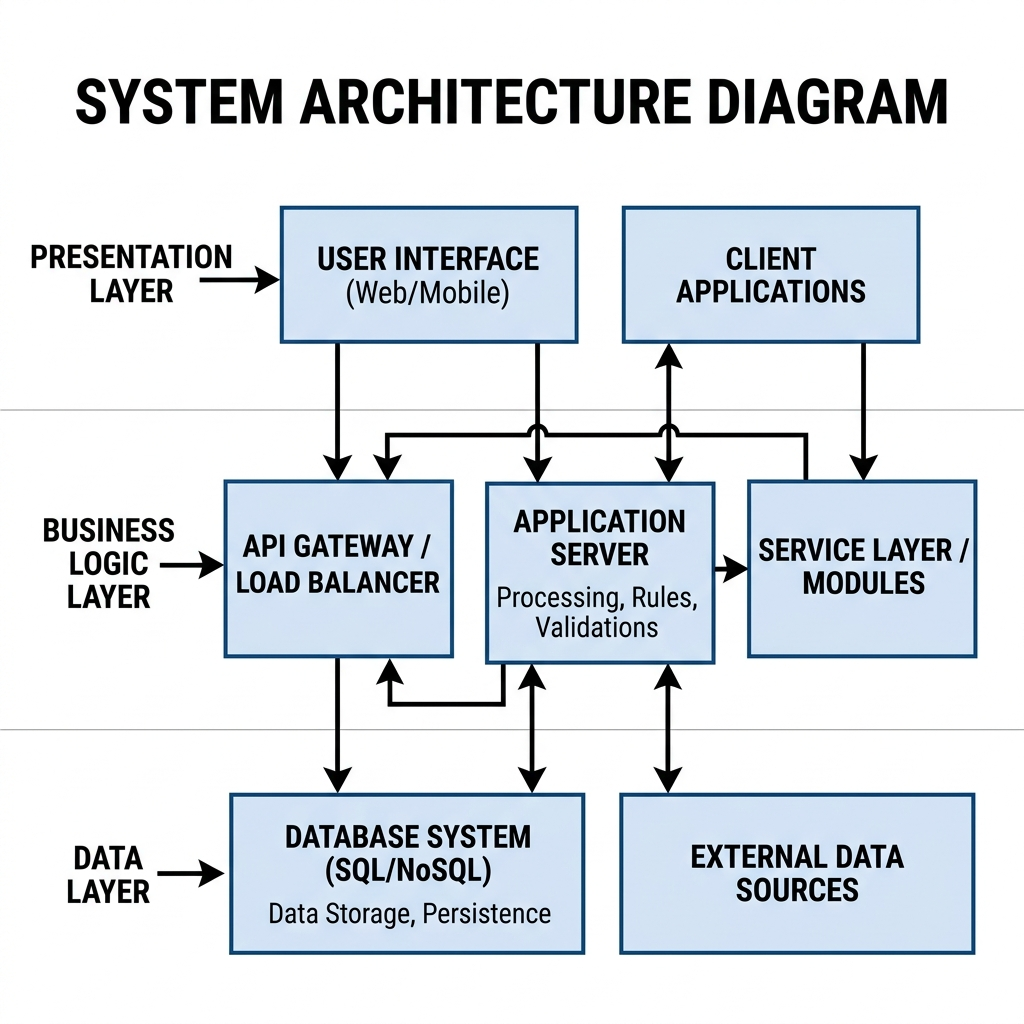
\includegraphics[width=0.92\textwidth]{system_architecture}
  \caption{Three-Tier System Architecture of Mitsuketa}\label{fig:sysarch}
\end{figure}

\section{Project Report Organization (Chapter Wise Summary)}
\begin{itemize}
  \item \textbf{Chapter 2 -- Literature Review:} Surveys existing media fingerprinting techniques, commercial systems, and academic research, and discusses their limitations.
  \item \textbf{Chapter 3 -- Problem Definition and Scope:} Formally defines the identification problem, project goals, constraints, and expected outcomes.
  \item \textbf{Chapter 4 -- System Requirement Specification:} Provides the system block diagram, use-case analysis, and hardware/software requirements.
  \item \textbf{Chapter 5 -- Proposed Methodology:} Describes the system architecture, mathematical modeling of fingerprinting algorithms, and the BK-Tree optimization strategy.
  \item \textbf{Chapter 6 -- Implementation:} Details the codebase structure, database schemas, API design, and the React frontend implementation.
  \item \textbf{Chapter 7 -- Results and Discussion:} Presents experimental test cases demonstrating system accuracy and robustness under various degradation conditions.
  \item \textbf{Chapter 8 -- Conclusion:} Summarizes the achievements of the project and outlines future directions for improvement and deployment.
\end{itemize}

\vspace{10mm}
\hrule